\documentclass[12pt]{article}
\usepackage{graphicx}
\usepackage{amssymb}
\usepackage{alltt}
\usepackage[pdftex]{hyperref}

\newcommand{\ic}{\texttt}
\newcommand{\firstref}{\textit}

\usepackage{alltt}
\usepackage{tex2page}

\newenvironment{code}%
   {\begin{alltt}}%
   {\end{alltt}}

\newcommand{\codeit}[1]{{\it #1}}
\newcommand{\codebf}[1]{{\bf #1}}
\newenvironment{float}%
   {\begin{center}}%
   {\end{center}
   }

\texonly   
\textwidth = 6.5 in
\textheight = 9 in
\oddsidemargin = 0.0 in
\evensidemargin = 0.0 in
\topmargin = 0.0 in
\headheight = 0.0 in
\headsep = 0.0 in
%\parskip = 0.2in
%\parindent = 0.0in
\endtexonly

%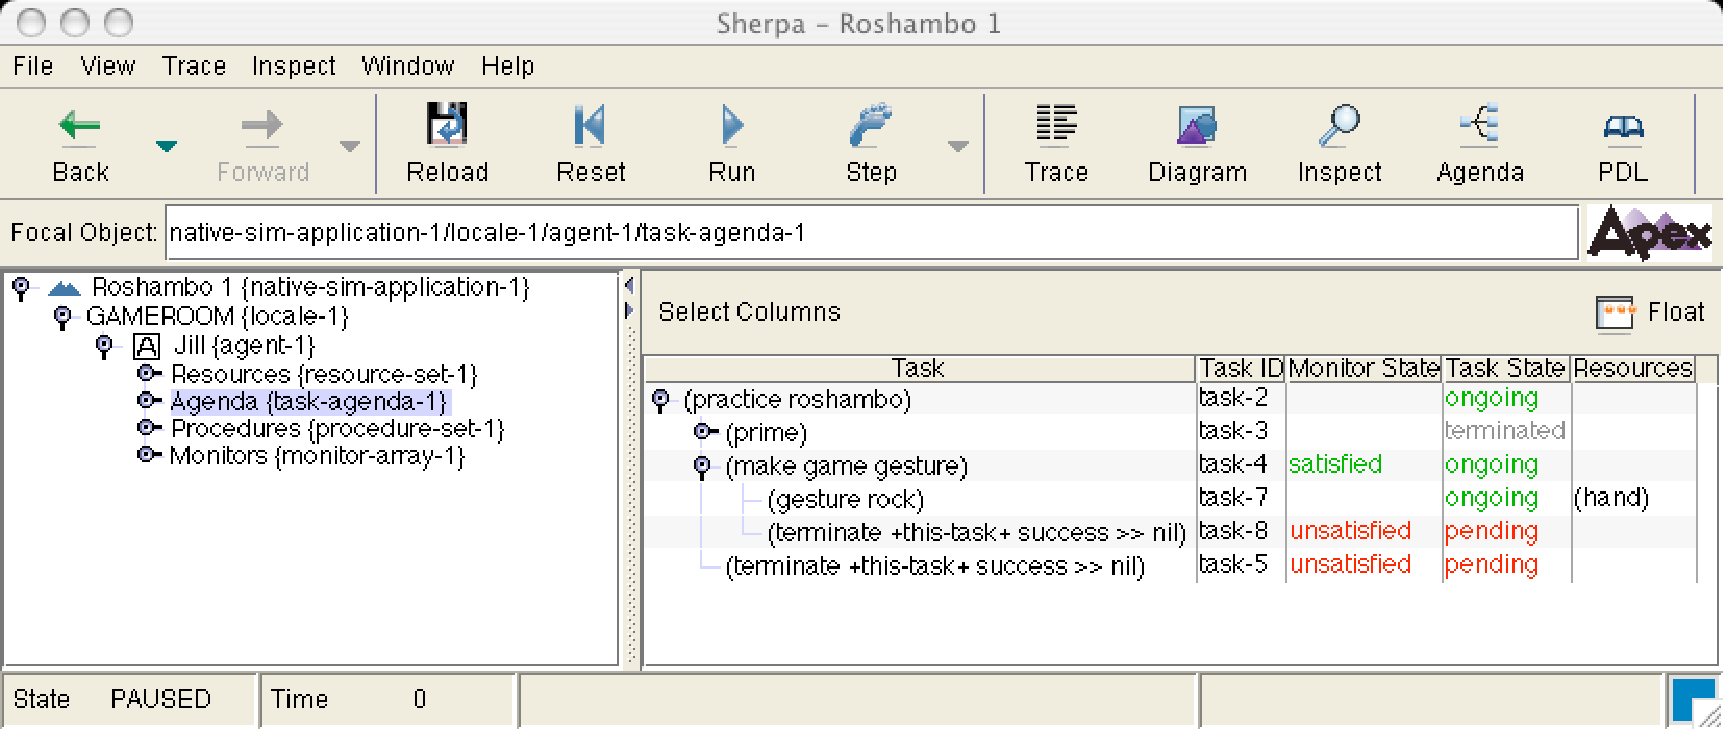
\includegraphics[width=6in]{sherpa-roshambo-1-1.pdf}


\newcommand{\img}[2]
 {\texonly \includegraphics[width=#1]{#2.pdf} \endtexonly
  \htmlonly \rawhtml <img src="#2.png"></img>\endrawhtml \endhtmlonly}

\htmlmathstyle{no-image}
\newcommand{\fn}[1]{\texonly\texttt{#1}\endtexonly
  \htmlonly \rawhtml <a href="#1"><tt>#1</tt></a>\endrawhtml \endhtmlonly}

\cssblock
body {margin-left: +5%; margin-right: +5%;
	 font-family: verdana, arial, sans serif; font-size:12pt; line-height:16pt }

td {font-family: verdana, arial, sans serif; font-size:12pt; line-height:16pt }
code, pre {font-family: "courier new", "courier";font-size:12pt; line-height:14pt }
h1 {font-weight:bold; font-family: verdana, arial, sans serif; font-size:14pt; line-height:18pt}
h2 {font-weight:bold; font-family: verdana, arial, sans serif; font-size:12pt; line-height:18pt}
h3, h4, h5, h6 { margin-left: +5%; font-weight:bold; font-family: verdana, arial, sans serif; font-size:12pt; line-height:16pt}
\endcssblock

\texonly
\title{\textbf{Paper covers Rock:\\An Apex tutorial}}
\endtexonly

\htmlonly
\title{Paper covers Rock: An Apex tutorial}
\endhtmlonly


\author{}
\date{}
\begin{document}
\maketitle
\htmlonly \rawhtml <center><img src="apexhome.jpg"></img></center>\endrawhtml \endhtmlonly

\tableofcontents
\newpage
\section{Roshambo}


Roshambo is another name for the game of ``Rock, Scissors, Paper.'' In Roshambo two players first ``prime'' the game by pumping their arms, and then make hand gestures of a closed fist (rock), forked fingers (scissors) or a flat hand (paper) for their play. The rules are ``Rock breaks scissors; scissors cut paper; paper covers rock," that is, rock beats scissors; scissors beat paper; paper beats rock; and if both players choose the same gesture, it is a tie. 

In this tutorial, we'll use Apex to develop successively more interesting versions of a simulated Roshambo match.

\htmlpagebreak
\section{Practice makes perfect: The basics of Apex}

Eventually, we'll have two players playing multiple rounds of Roshambo. But let's start small. Every Apex application needs:

\begin{enumerate}
\item a \ic{defapplication} form,
\item a Lisp initialization function that creates the application's agents, and describes each agent's initial goal,
\item at least one procedure for achieving the goal.
\end{enumerate}

\noindent In our first application, we'll just write the basic code for a player--the basics of what a player needs to play Roshambo. Figure~\ref{fig.roshambo.1} shows some Apex code for a one-player version of Roshambo--we'll call it Roshambo practice.

\begin{figure}
\begin{float}
\begin{code}
(defapplication "Roshambo 1"
    :init-sim (initialize-sim))

(defun initialize-sim ()
  (make-instance 'agent
    :name "Jill"
    :locale (make-instance 'locale :name 'gameroom)
    :initial-task '(practice roshambo)))

(procedure :sequential 
  (index (practice roshambo))
  (step (prime))
  (step (make game gesture)))

(procedure :seq
  (index (make game gesture))
  (step (gesture rock)))

(procedure :seq (index (prime)))

(primitive (index (gesture ?gesture))
  (profile hand)
  (duration (500 ms))
  (on-completion (inform `(gestured ,+self+ ,?gesture))))
\end{code}
\end{float}
\caption{Roshambo, Version 1.\label{fig.roshambo.1}}
\end{figure}

Notice that the \ic{defapplication} form gives our application a name \textit{Roshambo 1}, and tells Apex what initialization function to run to start the simulation.

The function is a Lisp function that does the basic requirements of any Apex application: 

\begin{itemize}
\item It creates an agent \ic{(make-instance 'agent ...)},
\item And places the agent in a locale \ic{(make-instance 'locale ...)},
\item And gives the agent an initial task \ic{:initial-task '(practic roshambo)}.
\end{itemize}

Notice, by the way, that the \ic{:init-sim} parameter to \ic{defapplication} tells Apex the create a simulation application. Real time applications are created using the \ic{:initapp} parameter. Since we're building simulated Roshambo agents, we want to use \ic{:init-sim}. 

The code for this first version of Roshambo can be found in the \ic{Apex:\-examples;\-roshambo;}\fn{roshambo1.lisp} file. Start Sherpa, and load this application. If you take the following steps:

\begin{enumerate}
\item Press the ``Step'' button.
\item Select ``Jill'' in the object hierarchy (the pane to the left).
\item Press the ``Agenda'' button.
\end{enumerate}

\noindent After following these steps, you should see something like Figure~\ref{fig.roshambo.1.1}, which shows the state of the Agenda as the agent, Jill, takes her ``priming'' step.

\begin{figure}
\begin{float}
\centerline {
%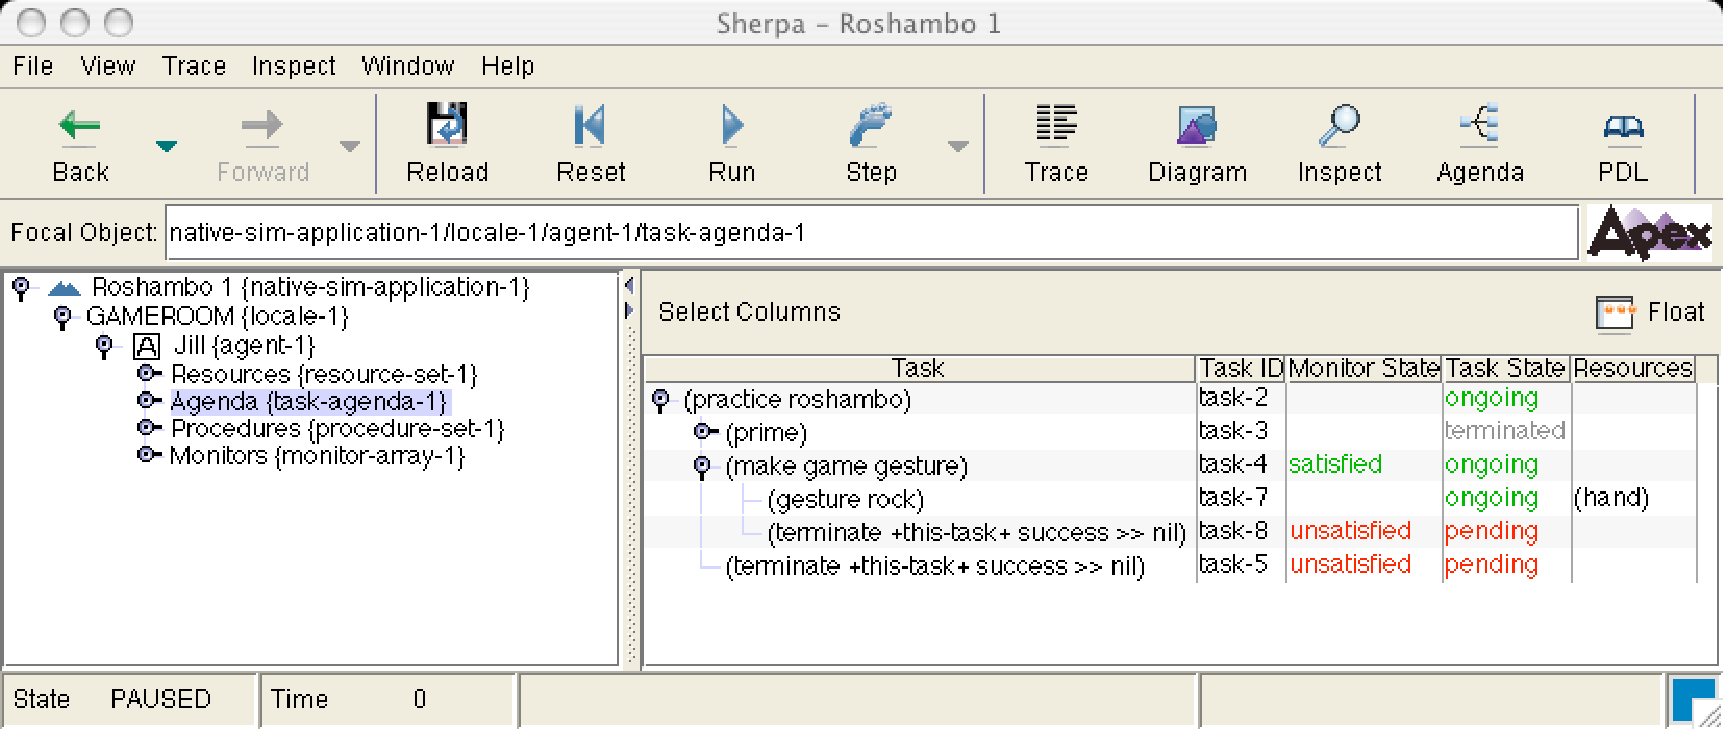
\includegraphics[width=6in]{sherpa-roshambo-1-1.pdf}
\img{6in}{sherpa-roshambo-1-1}
}
\end{float}
\caption{Agenda View of Roshambo, v1, after one step.\label{fig.roshambo.1.1}}
\end{figure}

There are just three procedures and one primitive in our first version of Roshambo. In Apex, a \firstref{primitive} define the basic actions that an agent can take. This is true for both simulations and real-time applications. The one primitive in this version of Roshambo, \ic{gesture}, uses the agent's (simulated) hand to make a gesture. We tell Apex that gesturing requires the \ic{hand} resource in the \ic{profile} clause. We tell Apex how long this action will take using the \ic{duration} clause. In simulations, the only way that time passes is by including durations in primitive forms, so it's a good idea to include a \ic{duration} for every primitive--it can be difficult to debug a simulation if many things are happening ``at the same time,'' which can occur if primitive actions don't take any time to transpire. The action taken by this primitive is to call the \ic{inform} function with the Lisp back-quoted list \ic{`(gestured ,+self+ ,?gesture)}. The special variable \ic{+self+} is always bound to the agent executing the task, and the variable \ic{?gesture} will be bound when the primitive \ic{(gesture ?gesture)} is called with a particular value. By the way, if we write \ic{`(gestured ,+self+ ,<?gesture>)}--\textit{i.e.}, with the variable surrounded by angle brackets--we'll get a warning if the variable is not yet bound. We'll use this convention in later versions.

The top-level goal for our agent is \ic{(practice roshambo)}. You may notice that Apex procedures and primitives look different from ordinary function calls in usual programming languages such as Lisp or C or Java. Apex uses \firstref{pattern matching} to find procedures and primitives to execute, so Apex can happily have \ic{index} clauses (which name the procedure or primitive) with spaces in them, and a name such as \ic{play roshambo} is different from a name such as \ic{play roshambo once}. Different people prefer different styles of naming--there's no particular reason not to name a procedure \ic{play-roshambo-once} as if it were a Lisp function. Some people think names like \ic{play roshambo once} make the code more readable. 

\begin{figure}
\begin{float}
\centerline {
%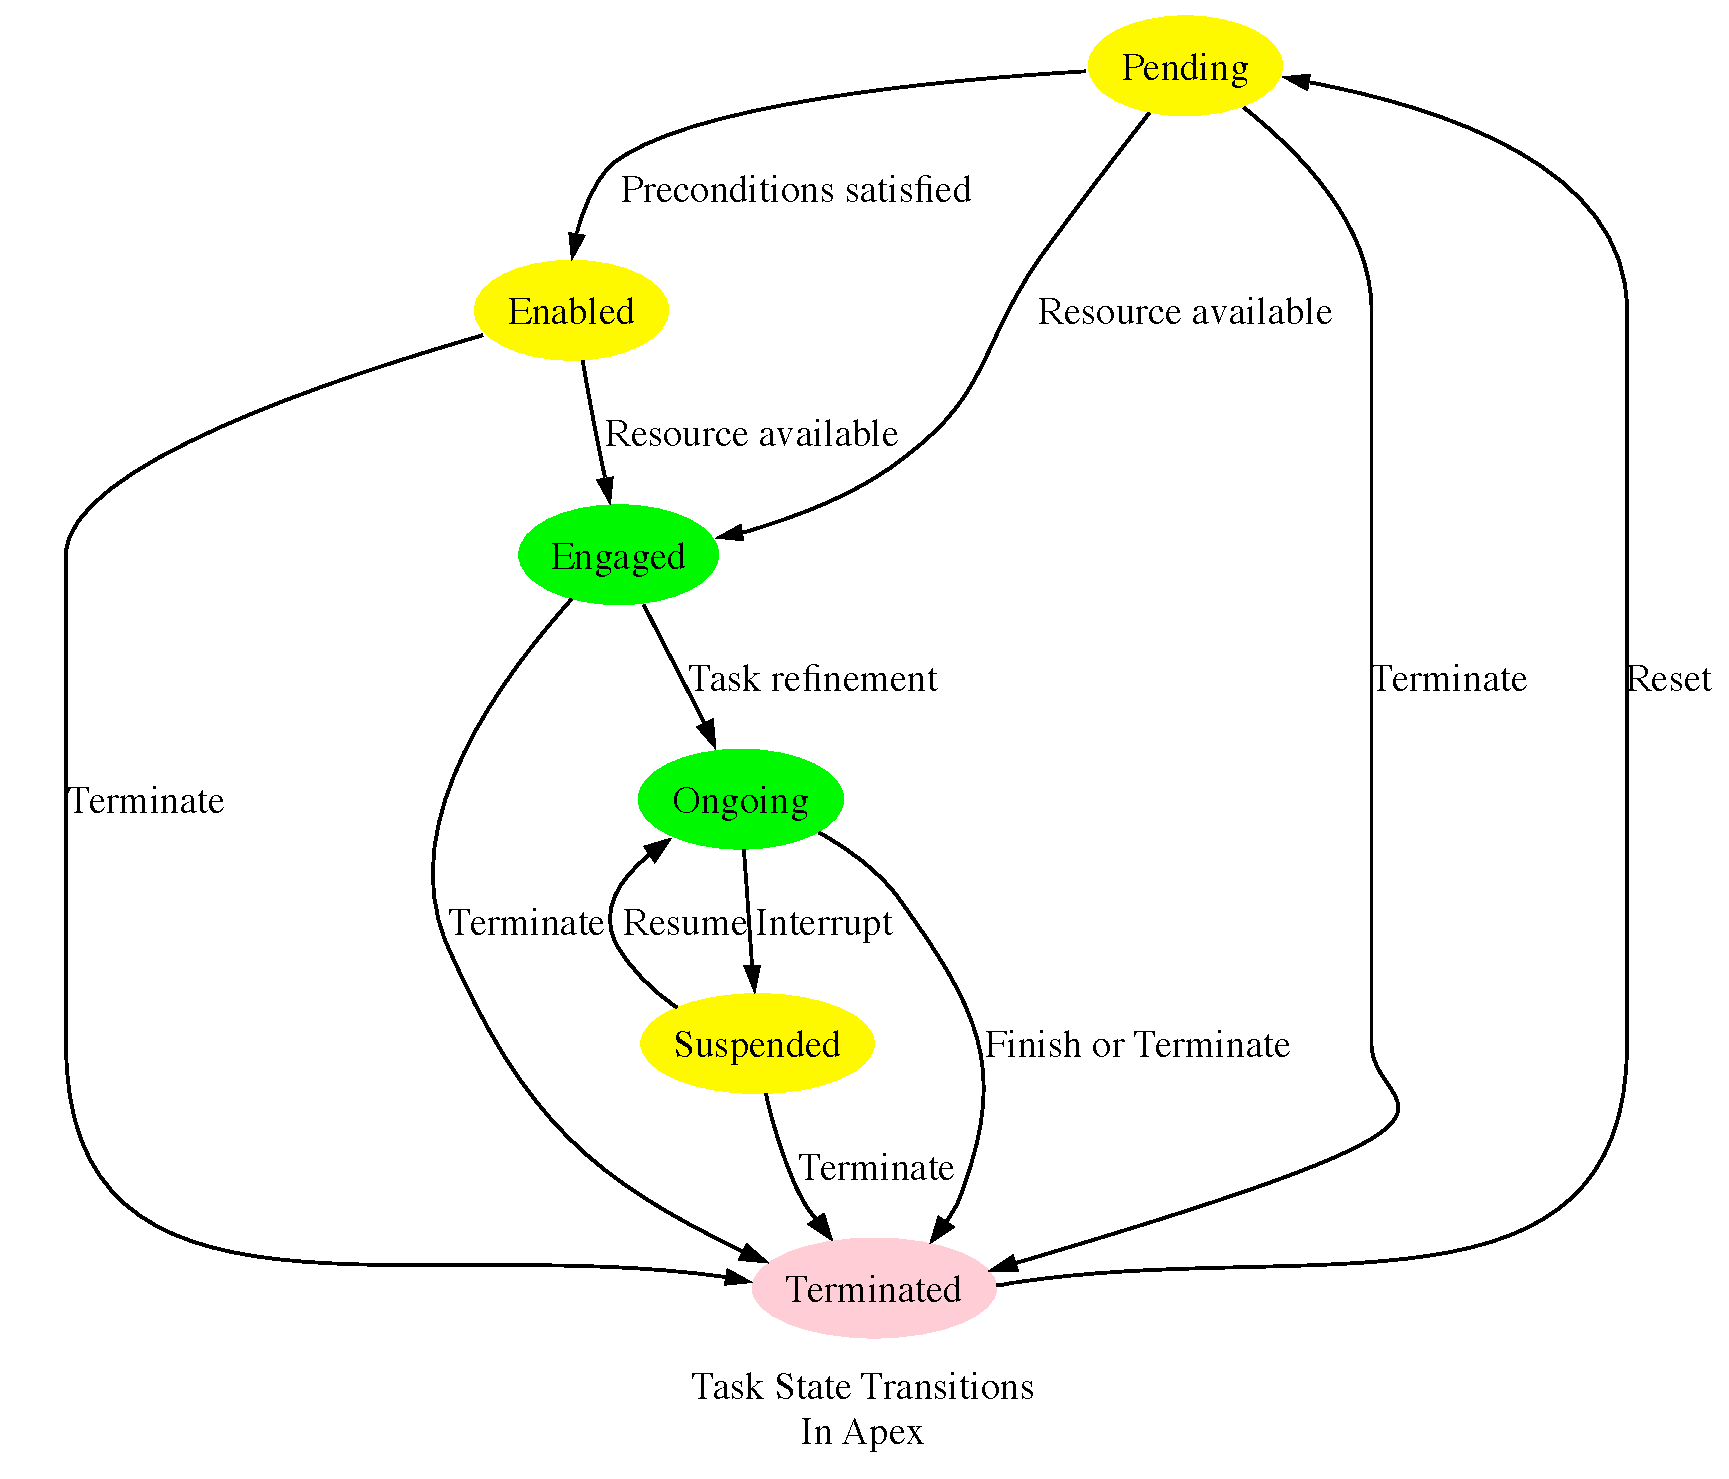
\includegraphics[width=6in]{tasktransitions.pdf}
\img{6in}{tasktransitions}
}
\end{float}
\caption{Task transitions in Apex.\label{fig.task-transitions}}
\end{figure}

The procedure  \ic{(play roshambo)} is declared to be \ic{:sequential}. (Later, we use a shortened form, \ic{:seq}, to declare the same thing.) This means the steps in \ic{(play roshambo)} are to be carried out sequentially--that is, the second step will not be enabled until the first step terminates, etc. Because sequential execution is the norm for most programming languages, it may seem odd to declare a procedure to be sequential. But the model of task execution underlying Apex is fundamentally based on the idea of multi-tasking, and so, unless specified, tasks are executed as soon as they are enabled.

``Enabled,'' and ``terminated'' describe different states that an Apex task can be in. Figure~\ref{fig.task-transitions} shows all of the possible task states a task can enter. When a task is created, it becomes ``pending.'' When its preconditions are met, it becomes ``enabled.'' When all resources it needs are available, it becomes ``ongoing''--that is, is it running. The task may be interrupted, in which case it becomes ``suspended.'' When it finishes, it becomes ``terminated.'' There are other ways for a task to become terminated. For example, if its parent is terminated, it will become terminated, so there is a line from every other state to terminated in Figure~\ref{fig.task-transitions}. Understanding how tasks can transition is very helpful in understanding what is going on in general. For example, it helps explain the ``task state'' column in the Agenda View in Figure~\ref{fig.roshambo.1.1}; the ``pending'' tasks are waiting for their preconditions to be fulfilled--in these cases, the completion of other steps.

\begin{figure}
\begin{float}
\begin{code}
(procedure :sequential (index (make game gesture))
  (profile hand)
  (step (gesture rock)))

(procedure (index (make game gesture))
  (profile hand)
  (step s1 (gesture rock))
  (step s2 (terminate) (waitfor ?s1)))
  
  (procedure (index (make game gesture))
  (profile hand)
  (step s1 (gesture rock))
  (step s2 (terminate) (waitfor (state ?s1 = terminated))) 
\end{code}
\end{float}
\caption{Three equivalent procedures.\label{fig.proc.equal}}
\end{figure}

Now, back to our Roshambo procedures. The procedure  \ic{(practice roshambo)} has two steps: \ic{(prime)} and \ic{(make game gesture)}. The  \ic{(prime)} procedure is very simple--there aren't even any steps! The \ic{(make game gesture)} procedure just has one step. We still include a \ic{:sequential} form to ensure they terminate. Note that the procedures in Figure~\ref{fig.proc.equal} are equivalent. The second step in the second version explicitly terminates the overall task when the first step terminates. In actually fact, the first version of the procedure is essentially shorthand (``syntactic sugar'') for the second version of the procedure.

But the second version of \ic{(make game gesture)} in Figure~\ref{fig.proc.equal} perhaps requires additional explication. Steps can be named or ``tagged''; the tags for the steps in the second version are \ic{s1} and \ic{s2}, respectively. The \ic{(terminate)} action in step \ic{s2} terminates the enclosing task; \textit{i.e.}, \ic{(make game gesture)}. The \ic{waitfor} clause describes the preconditions for step \ic{s2}'s enablement. 

This brings up another bit of syntactic sugar. Placing a variable with the same name as a step--as in \ic{(waitfor ?s1)}--is a shorthand for that step's being terminated, as in  the \ic{(waitfor (state ?s1 = terminated)} of step \ic{s2} of the \textit{third} version of the procedure in Figure~\ref{fig.proc.equal}. You'll see (and use) this shortcut time and time again in Apex procedures.

\htmlpagebreak
\section{Tell me about it: Communicating information between procedures}

Our second version of Roshambo is nearly the same. It seems a bit bogus that the \ic{(play roshambo once)} procedure should always gesture \ic{rock}. Figure~\ref{fig.roshambo.2} shows a new version of Roshambo, in which a primitive is called to choose a gesture. This can be found in \fn{roshambo2.lisp}.
\begin{figure}
\begin{float}
\begin{code}
(procedure :sequential 
  (index (practice roshambo))
  (step (prime))
  (step (choose gesture => ?my-gesture))
  (step (gesture <?my-gesture>)))

(primitive (choose gesture)
  (profile brain)
  (duration (500 ms))
  (return 'rock))
\end{code}
\end{float}
\caption{Roshambo, version 2. Changed procedures only.\label{fig.roshambo.2}}
\end{figure}

We introduce a new resource, simulating the use of the brain, in the gesture choosing primitive. Our agent still always chooses to gesture ``rock,'' but we have isolated the choosing to a separate task. 

The other thing of note in version 2 is how primitive communicates to a procedure that calls it. The \ic{return} clause sends a value, in this case, \ic{'rock}, to the calling procedure. THe value is captured into a pattern variable by using \ic{=>}; in this case, \ic{(choose gesture => ?gesture)}.

We also used the \ic{<?my-gesture>} form to help ensure that the variable \ic{?my-gesture} is bound before we use it.

\htmlpagebreak
\section{Two can play at this game: Multiple agents}

Of course, Roshambo is a game between two players, and currently we have only one player. Version 3 (\fn{roshambo3.lisp}) adds a second player, ``Jack'' to challenge our first player, ``Jill.'' At first, we'll have Jack and Jill choose gestures in exactly the same way, \textit{i.e.}, always choosing to play rock. Figure~\ref{fig.roshambo.3} shows that adding multiple agents is easy to do: we change the initialization function to do so.

\begin{figure}
\begin{float}
\begin{code}
(defun initialize-sim ()
  (let ((locale (make-instance 'locale :name 'gameroom)))
    (make-instance 'agent
      :name "Jill"
      :locale locale
      :initial-task '(practice roshambo))
    (make-instance 'agent
      :name "Jack"
      :locale locale
      :initial-task '(practice roshambo))))
\end{code}
\end{float}
\caption{Roshambo, version 3. Creating multiple agents.\label{fig.roshambo.3}}
\end{figure}

Because we want Jack and Jill to share the same location, we first create a \ic{locale} object before creating the agents. Because they have the same top level goal, they both prime and  gesture ``rock,'' and their done. Figure~\ref{fig.trace.roshambo.3} shows a trace of their actions. Here we are tracing the \ic{gestured} events--notice that the \ic{inform} primitive is informing all the agents of gestures, so that when Jack makes a ``rock'' gesture, both Jill and Jack receive a \ic{(gestured \#{agent-2 Jack} rock)}\footnote{To show the \ic{gestured} events in Sherpa, select the Trace view, press the Settings button on the Trace view toolbar, and select the \ic{gestured} checkbox under 'App' (Application) events.}. The forms in the left hand column show the time stamp and the agent--notice that choosing a gesture takes 500 ms., and gesturing takes 500 ms., so the ``run'' ends after 1 second (1000 ms).

\begin{figure}
\begin{float}
\begin{verbatim}
[0 Jill] (task-started #{task-2 (practice roshambo)})
[0 Jack] (task-started #{task-4 (practice roshambo)})
[0 Jill] (task-started #{task-5 (prime)})
[0 Jill] (task-started #{task-6 (choose gesture)})
[0 Jack] (task-started #{task-9 (prime)})
[0 Jack] (task-started #{task-10 (choose gesture)})
[500 Jack] (task-started #{task-11 (gesture rock)})
[500 Jill] (task-started #{task-7 (gesture rock)})
[1000 Jack] (gestured #{agent-1 Jill} rock)
[1000 Jill] (gestured #{agent-1 Jill} rock)
[1000 Jack] (gestured #{agent-2 Jack} rock)
[1000 Jill] (gestured #{agent-2 Jack} rock)
\end{verbatim}
\end{float}
\caption{Jack and Jill play version 3 of Roshambo.\label{fig.trace.roshambo.3}}
\end{figure}

\htmlpagebreak
\section{Bundles of joy: Providing different procedures for different agents}

Of course, it is a bit silly for Jack and Jill to have the same strategy of always playing ``rock.'' We can give agents separate libraries of procedures and primitives, called \firstref{bundles} by using the \ic{:in-apex-bundle} form. In the initialization function, we specify which bundles an agent has access to. In version 4 (\fn{roshambo4.lisp}), we'll specify that Jill always plays ''paper,'' and Jack always plays ''rock,'' by giving them different \ic{(choose gesture)} primitives. Any procedures or primitives defined before bundles are defined are shared by all agents. The changed code is in Figure~\ref{fig.roshambo.4}.

\begin{figure}
\begin{float}
\begin{code}
(defun initialize-sim ()
  (let ((locale (make-instance 'locale :name 'gameroom)))
    (make-instance 'agent
      :name "Jill"
      :locale locale
      {\bf :use-bundles '(:paper-strategy)}
      :initial-task '(practice roshambo))
    (make-instance 'agent
      :name "Jack"
      :locale locale
      {\bf :use-bundles '(:rock-strategy)}
      :initial-task '(practice roshambo))))
  
(in-apex-bundle :rock-strategy)    ;; always choose rock
(primitive (choose gesture)
  (profile brain)
  (duration (500 ms))
  (return 'rock))

(in-apex-bundle :paper-strategy)   ;; always choose paper
(primitive (choose gesture)
  (profile brain)
  (duration (500 ms))
  (return 'paper))
\end{code}
\end{float}
\caption{Roshambo, version 4. Using Bundles. Changed procedures only.\label{fig.roshambo.4}}
\end{figure}

\htmlpagebreak
\section{Fair play: Inter-agent communication}

Now we have multiple agents, but they don't know who has won the game.  We need a way for agents in Apex to communicate to one another. The normal way for this to occur in Apex is through the use of {\it routers}. A router is a ``publish-and-subscribe'' mechanism for agents; that is, agents subscribe to a router, and, when a message is published to the router, each subscriber receives the message. Agents can publish messages to routers they are subscribed to. Figure~\ref{fig.publish-and-subscribe} shows an example. As we said previously, agents are automatically  subscribed to a default router. The Apex Lisp function \ic{inform} sends messages to routers. When agents are created, they can be assigned a list of routers. Figure~\ref{fig.roshambo.5a} shows the new initialization code--note that the Lisp class for a router is {\it ps-router}. We'll give our agents a visual router (for gestures) and an auditory router (for spoken messages). Figure~\ref{fig.roshambo.5a} shows how the primitives \ic{gesture} and \ic{say} use \ic{inform} to send messages to their respective routers. The code can be found in the file \fn{roshambo5.lisp}. Notice that the \ic{say} primitive calculates the duration based on the length of the message (400 ms. per word).

\begin{figure}
\begin{float}
\centerline {
%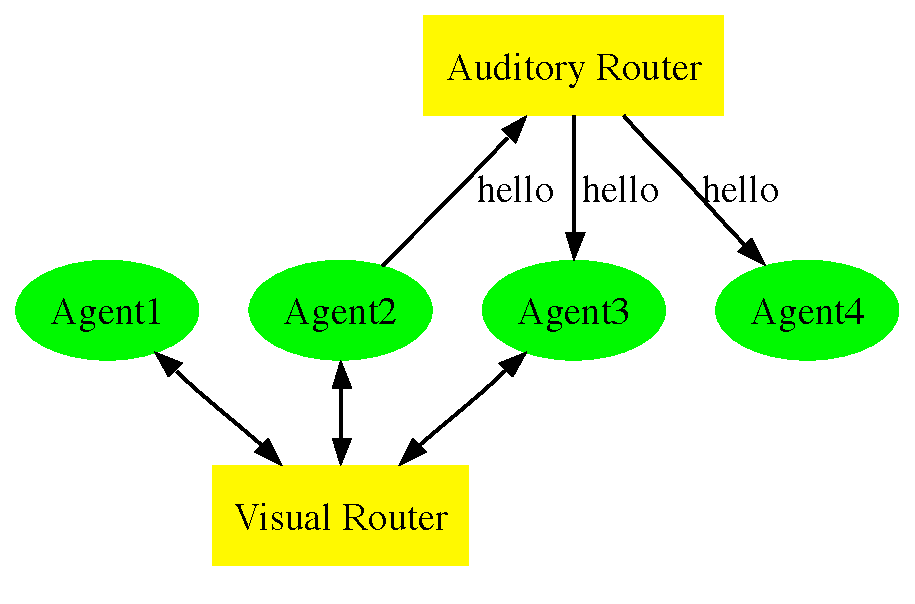
\includegraphics[width=4in]{agents-with-routers.pdf}
\img{4in}{agents-with-routers}
}
\end{float}
\caption{Publish and Subscribe Routers. The message Agent 2 published to the Auditory Router is passed to Agents 3 and 4. Agent 2 also receives the message. Agent 1, not a subscriber, does not receive the message.\label{fig.publish-and-subscribe}}
\end{figure}

Rather than have the agents merely practice Roshambo, Jack's goal is now to \ic{(play roshambo with jill)}, and Jill's goal is now to \ic{(play roshambo with jack)}. The basic plan for playing a game of Roshambo against an opponent is:

\begin{enumerate}
\item Prime and choose a gesture,
\item Make the play gesture,
\item When you see the opponent's gesture, determine the winner,
\item Declare the winner.
\end{enumerate}

In previous versions, we had our agents first prime, and then choose a gesture. But of course, there's no reason that our agents can't be thinking of a gesture as they are priming. Our simulation now has a bit of multi-tasking in it: they can potentially think and make a priming motion at the same time. (Well, the \ic{prime} procedure doesn't do anything yet, but we'll fix this soon). Figure~\ref{fig.roshambo.5b} shows the rest of the Version 5 code that has changed.

\begin{figure}
\begin{float}
\begin{code}
(defun initialize-sim ()
  (let ((locale (make-instance 'locale :name 'gameroom))
        (auditory-router (make-instance 'ps-router :name 'auditory-router))
        (visual-router (make-instance 'ps-router :name 'visual-router)))
    (make-instance 'agent
      :name 'jill
      :locale locale
      :use-bundles '(:paper-strategy)
      :routers (list auditory-router visual-router)
      :initial-task '(play roshambo with jack))
    (make-instance 'agent
      :name 'jack
      :locale locale
      :use-bundles '(:rock-strategy)
      :routers (list auditory-router visual-router)
      :initial-task '(play roshambo with jill))))

(primitive (index (gesture ?gesture))
  (profile hand)
  (duration (500 ms))
  (on-completion 
   (inform `(gestured ,+self+ ,?gesture)
     :router (router-named 'visual-router))))			    

(primitive (index (say . ?something))
  (profile voice)
  (duration (list (* (length ?something) 400) 'ms))
  (on-completion 
   (inform `(said ,@?something)
     :router (router-named 'auditory-router))))
\end{code}
\end{float}
\caption{Roshambo, version 5, showing initialization code and primitives for routing messages.\label{fig.roshambo.5a}}
\end{figure}

\begin{figure}
\begin{float}
\begin{code}
(procedure 
  (index (play roshambo with ?opp-name))
  (step (find agent ?opp-name => ?opponent))
  (step (prime)
        (waitfor <?find>))
  (step (choose gesture => ?mine))
  (step (gesture ?mine)
        (waitfor <?prime> <?choose>))
  (step (determine winner +self+ <?mine> <?opponent> <?other> 
         => (?winner ?winning))
	(waitfor ?gesture (gestured <?opponent> ?other)))
  (step (say winner is <?winner>)
	(waitfor <?determine>))
  (step (terminate)
	(waitfor <?say>)))

(primitive 
  (index (determine winner ?person1 ?gesture1 ?person2 ?gesture2))
  (profile brain)
  (duration (300 ms))
  (return 
   (determine-roshambo-winner ?person1 ?gesture1 ?person2 ?gesture2)))

(defun determine-roshambo-winner (person1 gesture1 person2 gesture2)
  (cond
   ((eq gesture1 gesture2)
    (list '|a tie| gesture1))
   ((or (and (eq gesture1 'rock)
             (eq gesture2 'scissors))
        (and (eq gesture1 'scissors)
             (eq gesture2 'paper))
        (and (eq gesture1 'paper)
             (eq gesture2 'rock)))
    (list person1 gesture1))
   (t (list person2 gesture2))))
\end{code}
\end{float}
\caption{Roshambo, version 5, playing procedures and primitives.\label{fig.roshambo.5b}}
\end{figure}

The interesting new things in Figure~\ref{fig.roshambo.5b} are (1) using routers to communicate between agents and (2) adding a bit of multi-tasking to our agents. Our procedure \ic{(play roshambo with ?opp-name)} is not strictly sequential, so we have to annotate steps so they don't begin until logically previous steps are completed. Figure~\ref{fig.roshambo.5b} shows yet another syntactic shortcut: if there is no tag name for a step, the tag name is created from the first form in the step's activity (so, for example, the default step name for \ic{(choose gesture => ?mine)} is \ic{choose}. (If multiple steps are created with the same first form, Apex will generate a name plus a number, \textit{e.g.}, \ic{choose-1}. It is probably best not to rely on steps automatically generated with numbers--give the steps names of your own choosing). 

We do a bit of Lisp programming in Version 5. In particular, we create a Lisp function to return the winner (or \ic{|a tie|} plus the winning or tying gesture as a list. We also use the standard primitive\footnote{Found in \ic{Apex:apexlib;default-apexlib.lisp}.} \ic{(find agent ?name)} to convert the name of an agent to the underlying data structure for the agent--this will mean the bindings of \ic{+self+} and \ic{?opponent} will has the same underlying form in call to \ic{(determine winner +self+ <?mine> <?opponent> <?other>)}.

\htmlpagebreak
\section{Prime time: Understanding when things happen}

Let's turn our attention to what seems like a minor thing, but will cause us a headache. We're going to break our application by adding one little seemingly innocuous line--understanding what goes wrong and why will make us better Apex developers. 

Here's the line we're going to add: we'll make the \ic{prime} procedure take one step, of making a priming gesture, like so:

\begin{code}
(procedure :seq (index (prime))
  (step (gesture priming)))
\end{code}

The file \ic{roshambo6-broken.lisp} contains this code. Running the code results in the trace shown in Figure~\ref{fig.roshambo.6.trace}. 

\begin{figure}
\begin{float}
\begin{verbatim}
[0 jill] (task-started #{task-2 (play roshambo with jack)})
[0 jill] (task-started #{task-5 (find agent jack)})
[0 jill] (task-started #{task-6 (prime)})
[0 jill] (task-started #{task-19 (gesture priming)})
[0 jill] (task-started #{task-7 (choose gesture)})
[500 jill] (gestured #{agent-2 jack} priming)
[500 jill] (gestured #{agent-1 jill} priming)
[500 jill] (task-started #{task-8 (gesture paper)})
[1000 jill] (gestured #{agent-1 jill} paper)
[1000 jill] (task-started #{task-9 (determine winner #{agent-1 jill} 
              paper #{agent-2 jack} priming)})
[1000 jill] (gestured #{agent-2 jack} rock)
[1300 jill] (task-started #{task-10 (say winner is #{agent-2 jack})})
\end{verbatim}
\end{float}
\caption{Jill loses to Jack who seems to have played ``priming''.\label{fig.roshambo.6.trace}}
\end{figure}


It's apparent that the \ic{determine winner} task is taking the \ic{priming} gesture as a move--even though Jack gestured \ic{priming} at 500 ms, and \ic{rock} at 1000 ms., which is when the \ic{determine winner} task begins. Recall that the \ic{determine winner} procedure has the following waitfor condition: \ic{(waitfor ?gesture (gestured <?opponent> ?other)}. 

Sherpa allows you to examine the state of monitors. To look at the state of this monitor when its conditions succeeded, take the following steps (assuming that the broken version 6 has run to completion):
\begin{enumerate}
\item Click on ``Jill'' in the object hierarchy (the panel to the left),
\item Press the ``Agenda'' button. 
\item Open up the agenda tree until the \ic{determine winner} task is visible.
\end{enumerate}

Notice that its monitor state column says the monitor has been satisfied. Hovering the cursor over the word ``satisfied'' shows a brief view on the monitor, but a more elaborate picture can be seen by:

\begin{enumerate}
\item Right-click\footnote{For the Macintosh, this is Apple-click, if you have a one-button mouse.} on the ``satisfied'' word in the monitor column.
\item Select ``Monitor diagram.''
\item In a little bit, you should see a diagram that looks something like Figure~\ref{fig.roshambo.6.broken.monitor}.
\end{enumerate}

\begin{figure}
\begin{float}
\centerline {
%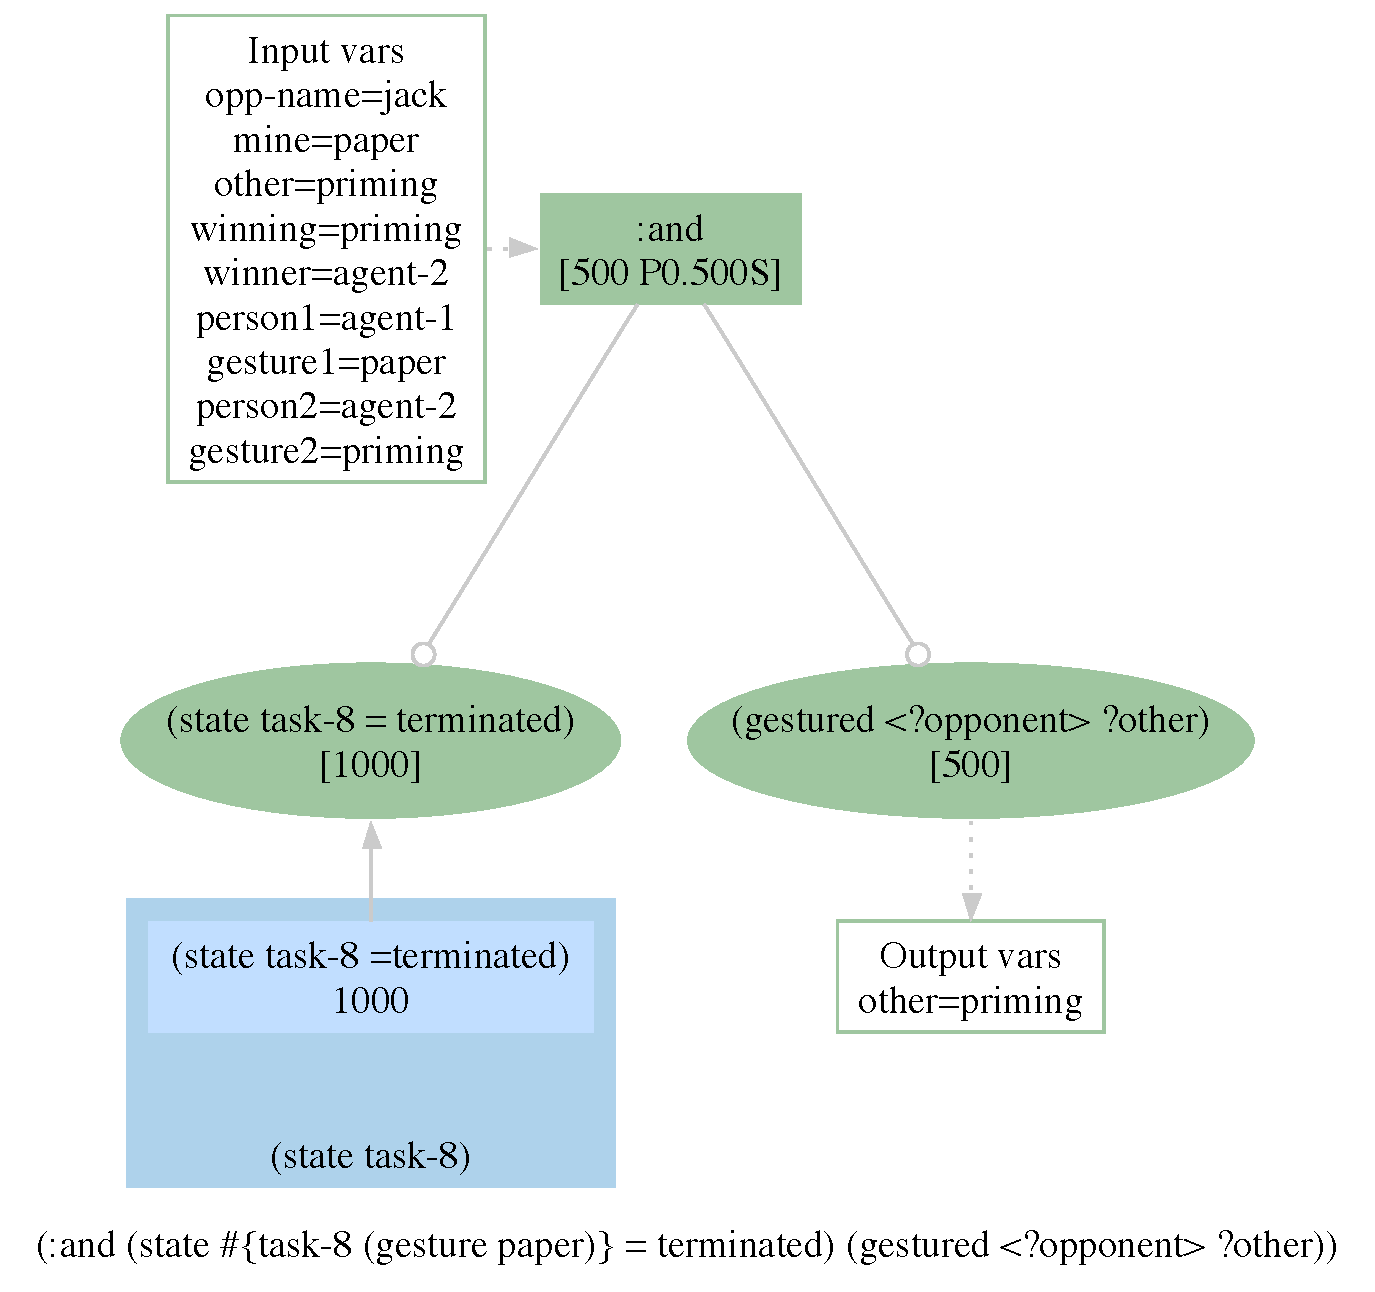
\includegraphics[width=4in]{roshambo6-broken.pdf}
\img{4in}{roshambo6-broken}
}
\end{float}
\caption{Visual representation of monitor from broken Version 6. Note that ``priming'' is an input value for variable \ic{?other} caused by the first \ic{gestured} event at 500 ms.\label{fig.roshambo.6.broken.monitor}}
\end{figure}

Apparently, ''priming'' is seen as the last gesture, even though we have set the steps up so that a game gesture occurs \textit{after} a priming gesture. What is happening here? 

Consider the five steps of procedure \ic{(play roshambo with ?opp-name)}. When this procedure is selected, all of these steps are created and their underlying tasks initiated. The monitor on the \ic{(determine winner)} step is created at the time the step gets created. Crucial to understanding the problem we have just encountered is this: \textit{monitoring for a condition always occurs within an interval of time}, either explicitly or implicitly defined. The implicit interval is always this: an interval beginning at the creation time of the monitor, and ending at infinity. In other words, monitors by default look for conditions that occur at or after the monitor is created.

Because the monitor for \ic{(gestured <?opponent> ?other)} is created at the same time that the \ic{(prime)} step is created, and the priming gesture is the \textit{next} gestured event that occurs, the monitor matches  \ic{(gestured <?opponent> ?other)} to \ic{(gestured \{agent-2 jack\} priming)}, binding \ic{?other} to \ic{priming}.

\htmlpagebreak
\section{A measured and orderly response: State variables and complex monitors}

The solution to our problem with Version 6 of Roshambo will first require us to understand how Apex works with data, either coming from its internal changes (such as the changing state of a task from pending to enabled, for example) or from other sources (such as the gestures of other agents, in our examples), which we'll call \firstref{sensors}. 

Sensors nominally create time-stamped data, with readings sometimes
done at constant intervals, sometimes not. Each reading provides a
time-stamped \firstref{measurement} of a \firstref{state variable}, that is, an
\firstref{attribute} of some \firstref{object} (often the agent, or a component
of the agent), which changes over time. 

Syntactically, measurements in Apex have the form \ic{({\it attribute} {\it object} = {\it value})}, where {\it attribute} {\it object} define the state variable of interest. In fact, we have already seen state variables used in monitors: monitors for termination of tasks, that look like \ic{(state {\it task} = terminated)}. Events like \ic{(gestured {\it agent} priming)} look very much like a measurement--but note the lack of an equals sign (\ic{=}). Other events--such as \ic{(said winner is a tie)}--look less like a measurement. Event forms that are not measurements are called \firstref{atomic episodes} in Apex. 

Since we are in control of the \ic{gesture} primitive, it is trivial to convert its gestures into measurements: now, the gesture primitive will emit forms with an equal sign, that is forms like \ic{(gestured {\it agent} = {\it gesture})}.

We can monitor for many different conditions, especially when these conditions are based on measurements of state variables. As a bonus, Sherpa offers a useful \firstref{state variable view} that shows the changing values of state variables over time, and the monitor views in Sherpa will do the same thing. In the present case, what we would like is to monitor for two things to occur \firstref{in order}: first the priming, then the game gesture. Apex provides monitoring capability for this and other conditions. In particular, we can use an \ic{:in-order} monitor to look for a priming gesture followed by a game gesture. Figure~\ref{fig.roshambo.6.fixed} shows the changed procedures; these can be found in file \fn{roshambo6-fixed.lisp}.

\begin{figure}
\begin{float}
\begin{code}
(procedure (index (play roshambo with ?opp-name))
  (step (find agent ?opp-name => ?opponent))
  (step (prime) (waitfor <?find>))
  (step (choose gesture => ?mine))
  (step (gesture <?mine>) (waitfor <?prime> <?choose>))
  (step (determine winner +self+ <?mine> <?opponent> <?other> => 
          (?winner ?winning))
          (waitfor ?gesture 
             \codebf{(:in-order
                    (gestured ?opponent = priming)
                    (gestured ?opponent = ?other))}))
  (step (say winner is <?winner>) (waitfor <?determine>))
  (step (terminate) (waitfor <?say>)))
             
(primitive (index (gesture ?gesture))
  (profile hand)
  (duration (500 ms))
  (on-start
   \codebf{(inform `(gestured ,+self+ = ,?gesture)}
	   :router (router-named 'visual-router))))
\end{code}
\end{float}
\caption{Changes to Version 6 to add an \ic{:in-order} monitor. Changes are highlighted.\label{fig.roshambo.6.fixed}}
\end{figure}

\subsection*{Other solutions}

There are some other possible ways to fix the \ic{(play roshambo with ?opp-name)} procedure, which we will sketch out here.

\begin{enumerate}
\item An additional condition could be added to the gesture step, viz., \ic{((gesture <?mine>) (waitfor <?prime> <?choose> \codebf{(gestured ?opponent = priming)}}. But will this work?

\textbf{It won't work.} Both the \ic{gesture} step and the \ic{determine} steps are created at the same time, and the \ic{(gesture \codeit{opponent} = priming)} measurement will be sent to both monitors. 

\item Perhaps one can force the \ic{gesture} step to be created later by creating a new subprocedure, something like Figure~\ref{fig.roshambo.6.poss.fix}. \textbf{Unfortunately this doesn't work either}--the tasks of a procedure are created ``at the same time,'' and  the tasks of a subtask are created ``at the same time.'' A little thinking will convince one that, for simulation applications at least, that these two times are, in fact the same time\footnote{In a real-time application, there will be real time passing, so the tasks will not, in fact, be created at the same time).}. 

\item Perhaps one can use an \ic{:or} monitor to monitor for just the right measurement. For example, \ic{(:or (gesture ?opponent = rock) (gesture ?opponent = paper) (gesture ?opponent = scissors))}. This will work, but there's a problem: you can't capture the opponent's move!\footnote{OK, I admit it, I tried to do this, and was chagrinned to see that I didn't have a binding for \ic{?other}.}

But there is a way to do this: we can place general constraints on monitors. 
\begin{code}
  (waitfor ?gesture 
   (:measurement (gestured <?opponent> = ?other))
   :constraints (member '?other '(rock paper scissors))))
\end{code}

\item The pattern matcher allows us to define constraints directly on values, using the special \ic{(?is \textit{var} \textit{predicate})} form. So, we can define a Lisp function \ic{(defun valid-p (x)
  (member x '(rock paper scissors)))}, and we can set the monitor in this way:

\begin{code}
  (waitfor ?gesture 
   (:measurement (gestured <?opponent> = (?is ?other valid-p))))
\end{code}

\end{enumerate}

\begin{figure}
\begin{float}
\begin{code}
(procedure (index (play roshambo with ?opp-name))
  ... 
  (step (det winner <?mine> <?opponent>)
   (waitfor (gestured <?opponent> = priming)))
  (step (terminate) (waitfor ?det)))

(procedure (det winner <?mine> <?opponent>)
  (step (determine winner +self+ <?mine> <?opponent> ...))
   (waitfor (gestured <?opponent> = <?other>))) ...
\end{code}
\end{float}
\caption{Putative changes to Version 6. Will this do the trick? (No).\label{fig.roshambo.6.poss.fix}}
\end{figure}

\htmlpagebreak
\section{Over and over and over again: Repeating tasks}

It's not much fun to play just one game of Roshambo, so let's allow our agents to play any number of games. The step-level clause \ic{repeating} provides a means to repeat a step while or until some Lisp condition is met. Because the condition is a Lisp condition, we need to set up a Lisp data structure to record the number of games a player has played. We'll just use a Lisp property list to record this. In addition, we'll need a new Apex primitive to increment the game count, and be sure to invoke this primitive after a game is played. Since we're are already saying who the winner is after a result is determined, we'll create a new procedure to do all the post-game work. This is version 7 of our Roshambo code; you'll find it in \fn{roshambo7.lisp}, and the changed procedures in Figure~\ref{fig.roshambo.7}.

\begin{figure}
\begin{float}
\begin{code}
(defparameter *games* (list))
(defun games (player) (or (getf *games* player) 0))
(defun (setf games) (val player) (setf (getf *games* player) val))

(procedure :seq
  (index (play roshambo ?n times with ?opp-name))
  (step s2 (play roshambo with ?opp-name)
    (repeating :until (>= (games +self+) ?n))))

(primitive (increase game count) 
  (duration 0)
  (return (incf (games +self+))))

(procedure 
  (index (record game ?mine ?opponent ?other ?winner ?winning))
  (step (increase game count))
  (step (say winner is <?winner>))
  (step (terminate)
    (waitfor ?increase ?say)))
\end{code}
\end{float}
\caption{Version 7 of Roshambo: Playing multiple games; changed procedures.\label{fig.roshambo.7}}
\end{figure}

Of course, we need to change the top-level goals of Jill and Jack to be \ic{(play roshambo 3 times with jack)} and \ic{(play roshambo 3 times with jill)}, respectively--with however many games we want them to play.

\htmlpagebreak
\section{Strategic decisions: Estimation monitors}

Our agents' Roshambo strategies are rather lame--Jill always plays paper, and Jack always plays rock. Let's give Jill a little more intelligence, and have her base her choice on the last gaming gesture by Jack--if he played rock last time, she'll play paper this time, if paper, scissors. Of course, Jill will have to make a choice based on some other strategy the first time she plays, because she'll not have a history to base her decisions on.

As in the previous section, we'll have to be careful to distinguish between game gestures and priming gestures. It's a bit of a pain to distinguish between regular gestures and game gestures, so as part of the \ic{(record game)} procedure, we'll have the agent tell itself the game gesture of the opponent as a measurement; that is, \ic{(game-gesture opponent = \textit{gesture})}. We'll also  take a slightly different tack--we'll view the values of the \ic{(game-gesture oppoenent)} state variable as persisting. That is, we'll assume that once a player has made a gesture, that gesture remains relevant until another gesture comes along. In doing so, we treat the measurements of a state variable as a \firstref{fluent}, that is, a proposition that remains true until a new value comes along. In Apex's terminology, this kind of condition is called an \firstref{estimation}--that is, in this case, we are estimating that the value of a state variable at some time $t$ was the last measurement made at or before $t$. Apex provides two kinds of estimation monitors: \firstref{persistence} monitors and \firstref{regression-based} monitors. What we want is a persistence monitor for Jill. In general, we can control how long a persistence monitor's estimation will be considered to hold; for Roshambo, we'll assume it will hold forever. 

Figure~\ref{fig.roshambo.8} shows the changed code for Version 8 of Roshambo--in addition, of course, we have to initialize the Jill agent with this bundle. The entire application can be found in \fn{roshambo8.lisp}.

The \ic{choose gesture} procedure for Jill is as complicated a procedure as we have seen. Basically, it sets up two tasks that compete in parallel, and, given the nature of the underlying data, only one with succeed. The two cases are if the opponent hasn't made a previous game gesture, and if the opponent has made a previous game gesture. If the opponent hasn't made a game gesture yet, there will be no measurement of it, we check whether it is not the case that a measurement was made since ``the beginning of time,'' (remember, we're assuming that game gestures persist). In this case, we'll choose a gesture randomly.

If the opponent has made a game gesture, there will be a measurement--and we use a \ic{:persist} estimator to find it. In this case, we'll call an ``expert'' to decide the gesture based on that last gesture--this is a pretty simple expert, so we can encode it in a primitive clause.

\begin{figure}
\begin{float}
\begin{code}
(primitive (remember (?attr ?obj) = ?value)  
  (duration (500 ms))
  (on-start
   (cogevent `(,?attr ,?obj = ,?value) +self+)))

(in-apex-bundle :beat-last-strategy)

(defun random-elt (lst) (elt lst (random (length lst))))

(primitive (choose gesture randomly)
  (profile brain)
  (duration (500 ms))
  (return (random-elt '(rock paper scissors))))

(primitive (choose gesture by last ?last)
  (profile brain)
  (duration (500 ms))
  (return (ecase ?last (rock 'paper) (paper 'scissors) (scissors 'rock))))

(procedure (choose gesture)
  (step s1 (choose gesture randomly => ?gesture)
    (waitfor (:not (:measurement (game-gesture opponent = ?)
                    :timestamp (> 0)))))
  (step s2 (choose gesture by last ?last => ?gesture)
    (waitfor (:measurement (game-gesture opponent = ?last)
                :estimation (:persist))))
  (step (terminate >> ?gesture)
    (waitfor (:or ?s1 ?s2))))
\end{code}
\end{float}
\caption{Roshambo version 8, \ic{:beat-last-strategy} bundle.\label{fig.roshambo.8}}
\end{figure}



\htmlpagebreak
\section{Game for more: Next steps in Apex}

We started with a simple practice game of Roshambo, and now we have two agents playing each other multiple times, using different strategies. Perhaps you can think of other strategies to implement. The Apex Manual contains the reference material you'll need. And if you come up with a killer new Roshambo strategy--let us know!


 \end{document} 